\section{Field Study}
A small-scale study was conducted which ran for 3 weeks and included 10 participants (including the author). In the study the participants used the application discussed in Chapter \ref{chapter:05} that collected their location data and computed mobility features daily. This section will discussed the overall method with which the study was conducted.

\subsection{Self-study}
Before the main study was conducted a self-study was conducted in three different cities, in order to select appropriate parameters for the algorithms. This parameter tweaking happened while the author was in Munich where he sat in a large university building and visited different offices. In Figure \ref{fig:tum-map} the Places and the Stops at the university are displayed and as can be seen which are very close. Had the radius parameter for finding places been higher then some the places would have been merged into a single place. Here, the parameter was set to 25 meters, and in the final study it was chosen to set it to 50 meters.

\begin{figure}
    \centering
    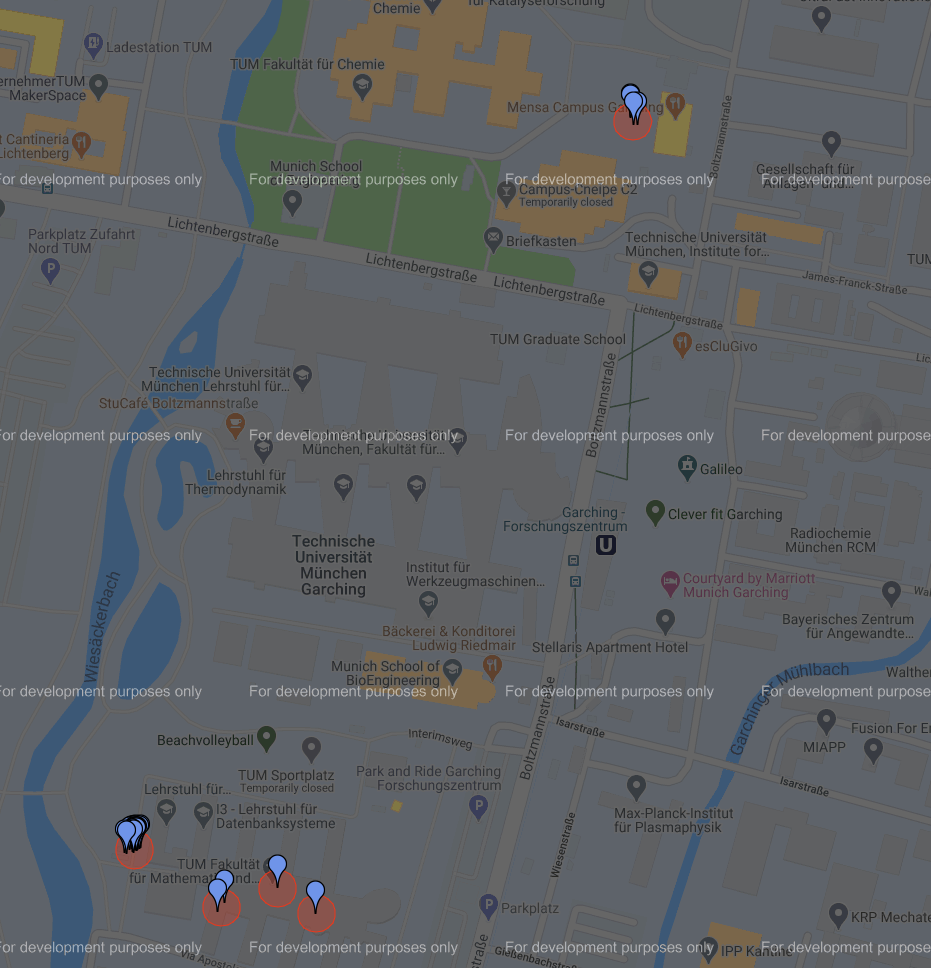
\includegraphics[width=0.7\textwidth]{images/map/map-tum.png}
    \caption{A map of TUM Garching, displaying the Places (red clusters) as well as the Stops which make up these places (blue markers) visited by the author}
    \label{fig:tum-map}
\end{figure}

\subsection{Main Study}
In addition to this the application also had a diary consisting of 4 questions that the user had to fill out each day. In order to make it easy for the user to remember filling out the diary, a reminder was sent to the participants at 8 PM. The time 8PM was chosen due to being relatively late while still being early enough in the day that people would still be checking their phone. Some people go to bed at 9-10 PM which had to be taken into account. The diary questions were related to 3 of the Mobility Features which were \textit{Number of Clusters}, \textit{Home Stay} and \textit{Routine Index}. The point of the questions were to get a subjective estimates of the values of these features. It is important to stress the fact that these these answers are estimates since the user cannot be expected to give very precise answers and secondly they are very subjective since the definition of things such as a 'Place' may vary a lot from person to person.

\subsection{Evaluating Features}
Answers were collected through a diary in order to evaluate, to choose the most important parameters certain features were evaluated through comparing subjective answers with calculated features. The features had to be ease to formulate as a question such that subjective user answers could be collected, as such features such as entropy and location variance were ill-suited, whereas Home Stay, Number of Places and Routine Index were chosen instead. The questions the user was asked were the following:

\begin{itemize}
    \item[\#1] How many unique places (including home) did you stay at today?
    \item[\#2] How many hours did you spend away from home today? (Rounded-up)
    \item[\#3] Did you spend time at places today that you don't normally visit?
    \item[\#4] On a scale of 0-5, how much did today look like the previous, recent days? (Where 0 means 'not at all' little and 5 means 'Exactly the same')
\end{itemize}

\textit{Where question \#3 and \#4 relate the Routine Index feature.}

Collecting the subjective \textit{number of places} visisted, was done by asking the participant exactly that, making it the easiest of the 3 features to evaluate. For collecting the subjective \textit{Home Stay} percentage, the user was asked the inverse question, i.e. how many hours they were \textit{away} from their home today (from which Home Stay can then be calculated later). This question is much easier for the participant to answer, and there is no need to explain to the user that time spent during the night counts towards the Home Stay, as an example. The Routine Index was more difficult to formulate as a question since there is no succinct way of putting it. It was decided upon rating today scale from 0 to 5, where 0 indicates that today looks nothing like previous days and 5 indicating that today looks identical to the previous days. Ideally the scale should be more fine grained such as 0 to 10, however this put too much on the user, the main information we wished to draw from the user was a very high level overview of whether the day today was a lot like the previous days. Question \#3 also related to the Routine Index feature but was not used for later data analysis since it was hard to compare directly to the Routine Index and would require looking at the Hour Matrix instead.

\subsection{The Impact of COVID-19}
The Corona virus pandemic lead to countries closing borders and urging people to stay at home as much as possible. This included workplaces shutting down and people had to work from home, as well as places of recreational character such as gyms and restaurants. This had some major implications for the study and meant that it would be expected that the participants routine was quite steady, since they were mostly home, and that the home stay percentage was very high and that the number of places visited was very low. In addition it was probably also not common for most people go visit new places during the pandemic. However, all in all the pandemic only shaped the results of the field study and did not prevent the study from taking place at all.


